\documentclass{evolang12}
\usepackage{graphicx}
\usepackage{float}
\usepackage{url}
\usepackage{authblk}
\usepackage{amsmath,mathtools, amsthm, amssymb}
\DeclareMathOperator*{\argmin}{arg\,min}
\DeclareMathOperator*{\argmax}{arg\,max}
\begin{document}


\title{GEN.DLANG: A COMMUNITY GENERATED DESIGN LANGUAGE}
\author[*1]{ANONYMOUS AUTHOR 1}
\author[2]{ANONYMOUS AUTHOR 2}
\affil[*]{Corresponding Author: name@domain.com}
\affil[1]{This Department, University X, City, Country} % Center for Design Research, University of Kansas, Lawrence, USA
\affil[2]{That Department, University Y, City, Country} % HAMZA's affiliation...
% \affil[3]{Other Department, University Z, City, Country} % HAMZA's/Erick's additional affiliation...

%%%%% INSTRUCTIONS FOR ADDING AUTHORS %%%%%

%Initial submissions should be anonymous - DO NOT INCLUDE ANY IDENTIFYING INFORMAITON IN THE SUBMISSION VERSION -(i.e., no author details should be added above). To avoid problems with page limits, please include the appropriate number of placeholders for authors. If multiple authors share an affiliation, they can be paired with the appropriate affiliation using the numbers in the square brackets next to "author" and "affil" to save space. Designate a single corresponding author using the asterisk.

%%%%% INSTRUCTIONS FOR ADDING AUTHORS %%%%%

% HAMZA-0: Could you please make sure we follow all of the guidelines according to:
% http://evolang.org/submissions

\maketitle

\paragraph{Introduction}
\frenchspacing
This design project aims to integrate ideas from cultural evolution, machine learning, and generative design to construct a conceptual foundation of language evolution. Through the use of genetically-inspired optimized automatic speech recognition-hidden Markov models (GMM-ASR-HMM) and generative adversarial networks (GAN), people independently input personal aesthetic preferences to generate geometric visualizations. The design system runs on a mobile Linux-based computing system, where individuals choose the characteristics of the symbol displayed (i.e., color, complexity, shape, and amount) through a graphical user interface. In doing so, participants collaborate with and contribute to an ever-evolving design by providing individual input into the system's growing collection of preferences. The aggregated preferences reflective of the communities' aesthetic value are captured as a latent variable in the mathematical model. This design system can be generalized to track and model other forms of language evolution.

\paragraph{Cultural Evolution}
The history and identity of a culture-community is regularly fossilized as artifacts generated by its participating members \cite{dor2015instruction,ferdinand2015inductive}. Such enduring cultural artifacts are resilient, surviving through replication from individual to individual and generation to generation. Over time, elements are naturally added, subtracted, substituted, and rearranged as they are transmitted from mind to mind \cite{ferdinand2015inductive}. Of course, culture is often materialized into \textit{physical structures} in the form of art or architecture, which are the fruits of human cognitive and physical labor. However, it is the ideas or stories embodied in these artifacts that are truly subject to mutation and transmission, and provide inspiration for new structures and theories. More commonly, cultural artifacts are entirely social and immaterial, evolving through time as in the case of natural languages like Arabic and English \cite{ferdinand2019cognitive,dor2015instruction}. 

\paragraph{Mathematical Model}
In order to perform \textit{automatic visualization generation} (AVG), one must build the appropriate mathematical model. \textit{Hidden Markov models} (HMMs) are a pervasive statistical tool used for similar applications in a variety of fields. In fact, HMMs are known for modeling all sorts of sequential pattern processing and classification problems through a doubly stochastic process. One of the stochastic processes is a hidden sequence of states (Markov chain) that produce a sequence of random \textit{observable symbols}. This sequence of observable symbols are then governed by another stochastic process. In our design system, the observable symbols are aesthetic preferences and the hidden states are the visualizations. In general, this process can be viewed as building computational modules, where at the crux is the decoder. In fact, this design system utilizes an ASR-based HMM framework \cite{gales2008application,young2002htk} which was originally designed for automatic speech recognition. 

More recently, deep learning researchers have found great success in generative design through the use of Generative Adversarial Networks \cite{NIPS2014_5423}. A GAN is actually a combination of two competing neural networks. The first network, called the generator, takes in random numbers and produces new data instances while the second network, called the discriminator, evaluates whether this instance belongs to the original training data set. Thus, they train each other through a double feedback loop, the discriminator learning important features from the real data and the generator learning important features from the discriminator. The end result is a generator that produces realistic data.


\paragraph{Design Approach}
GEN.DLANG attempts works to generate the most preferred or fittest visualization as a function of public interactions. The system attempts to infer novel output (visualization) from random input (preference information), and a collection of environmental and internal constraints. More, the design system works to incorporate learning into the generation of the default design by learning over the collected design characteristics from within the sets \textit{complexity} $C$, shape $P$, color $RGB$, and size $S$:
\begin{equation}
NORM &= C \cup RGB \cup P \cup S
\label{eq:third-phase}
\end{equation}
Thus, users specify their visualization preferences, the system makes a copy or memory of these preferences, saving it into a collection of preferences, $NORM$. For example, one preference might be a higher weight or frequency of blue colored shapes, or conversely, a lower number of complexities will be selected out of for if low complexity is less frequent in $NORM$. As a result, the fittest individuals and resulting generated design language is some set of preferences that ascribes to this fit collection. Practically, this system is running on a Raspberry Pi, which runs the Python code for learning, the pj5 code for visualization, JavaScript code for web deployment, and connects a dynamic microphone and multimedia projector via HDMI as shown in the figure.

\begin{figure}[!htbp]
 \centering
 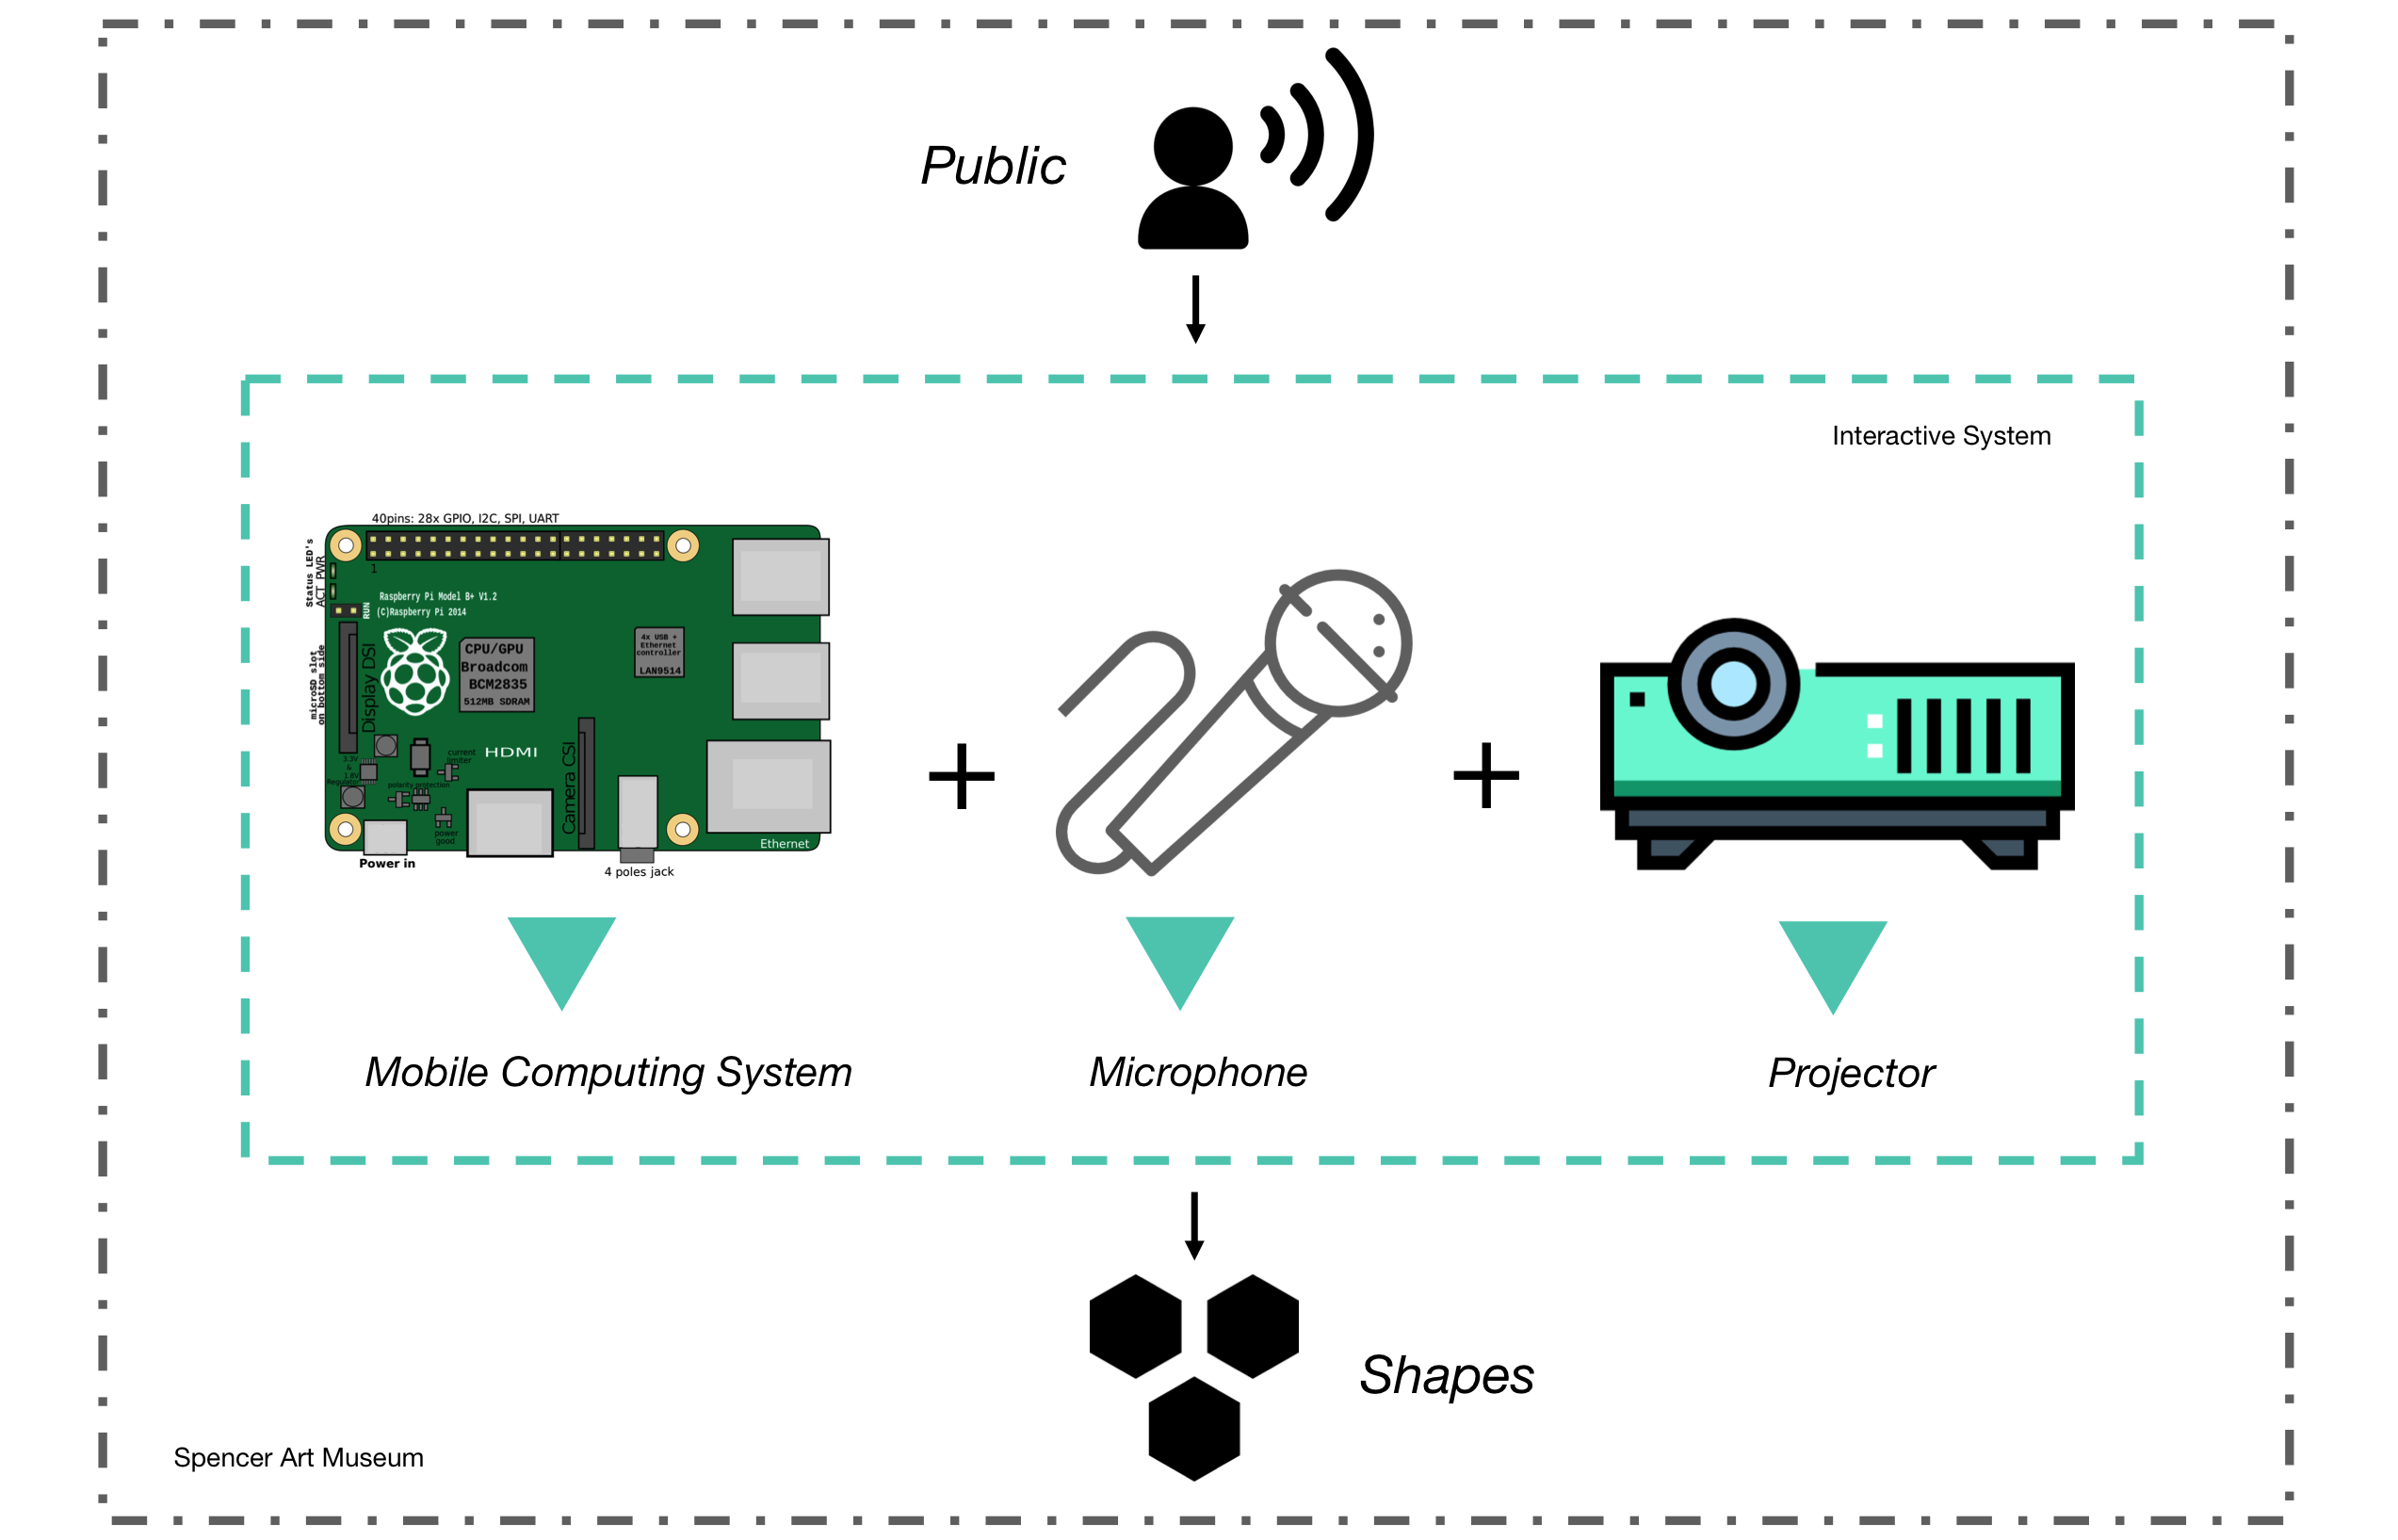
\includegraphics[width=0.90\textwidth]{EvoLang12-SPENCERDESIGN.png}
 \caption{The interactive design system consist of a mobile computing system (Raspberry Pi), a USB microphone, and a multimedia projector. The public provides input data which is then processed by the computing system to generate various shapes and novel structures throughout the day}
 \label{EvoLang12-SPENCERDESIGN.png}
\end{figure}
\newpage

% \paragraph{First Phase}
% The \textit{first design phase} uses pre-defined specification for the \textit{color}, \textit{complexity}, \textit{shape}, and \textit{size} of the visualization components. Particularly, the colors of the shapes in the visualization are some values from within the RGB range, the shapes are chosen to be boxes  from the set $\in$ $\lbrace box, ellipse, sphere \rbrace$ which correspond to the pre-defined shapes in the \textit{processing programming language} \cite{reas2006processing}. In truth, this first phase is simply a base or bootstrap for the consecutive phases. Hence, this basic form allows the most concrete specification of the sound-based visualization. This phase does not incorporate any learning, and it simply a product of one individual preference.

% \paragraph{Second Phase}
% The \textit{second phase} works to create a more general visualization where the components (or specifications) can be chosen at anytime by the user. Thus, the complexity can be chosen from some value $\in$ $ C = \lbrace c_1, c_2, \ ... \ , c_n \rbrace$, and the colors can be chosen from some value $\in$ $RGB = \lbrace u_1, u_2, \ ... \ , u_n \rbrace$, and the shapes can be specified from $\in$ 
% $P = \lbrace s_1, s_2, \ ... \ , s_n \rbrace$, and finally the size of the \textbf{visualization} can be some value chosen $\in$ $ S = \lbrace size_1, size_2, \ ... \ , size_n \rbrace$. 

% \subsection{Design System Software}
% The system was written in the programming languages, \textit{Python} and \textit{Processing}. Specifically, the pj5 flavor of Processing was used to create the web-based visualization that is accessed by some Linux-computing system, which is connected to an output display via HDMI. The GA-ASR-HMM are written in Python and \textit{JavaScript} with its associated node.js packages. JavaScript was chosen for its flexibility and ease of implementation for hosting this visualization online. 

% \subsection{Design System Hardware}
% Practically, this system is running on a Raspberry Pi, which runs the JavaScript code for learning, the pj5 code for visualization, and connects a dynamic microphone and multimedia projector via HDMI. In theory, the system can be implemented on various computing platforms and associated operating systems; the Raspberry Pi was chosen because of its hardware specifications, in particular its networking and processing capabilities, as the visualization happens at 60 FPS. Hence, this system can be interpreted on any operating system that has such networking capabilities, sufficient storage, and the necessary peripherals and shown in Fig.~\ref{EvoLang12-SPENCERDESIGN.png}. 

% HAMZA-3: Could you please write a paragraph about using such a system to generate art in the style of notable artist
% HAMZA Notes: Please pay attention to the Design System Software and System Hardware section...
% subsection{Application of System}


% \section{Conclusion}
% Presented in this document is a design system framework that attempts to generate the most preferred or fittest visualization as a function of public interactions. The system is inspired from basic cultural evolution concepts and entertainment applications of the fast Fourier transform. In the end, this system attempts to infer novel output (visualization) from random input (acoustic information), and a collection of environmental and internal constraints. This process is undertaken through a combination of Fourier analysis and genetically-optimized hidden-Markov models. As such, the focus of this system is  not necessarily providing an accurate representation of human cognition, and instead a framework for inferring and constructing structural representations for a learned public space.

% HAMZA-4: So after you read it trash this shit. Like the more scrutiny the better. Additionally, below are the section and subsection guidelines for this EvoLang12 Submissions. Please, take a look at these to make sure we're following everything.

% HAMZA-5: Please add or suggest any sections we should write

% ERICK: Make appropriate changes that Hamza suggest: sections, subsections, figures, etc.

% \section{Guidelines}

% \subsection{General Guidelines}

% We have provided eight files for use when producing a paper using latex. 

% \begin{enumerate}

% \item {\em evolang12.tex} --- the source for this document. 

% \item {\em evolang12.pdf} --- PDF generated from {\em evolang12.tex}.

% \item {\em evolang12.png} --- the figure file.

% \item {\em evolang12.bib} --- the bibliography file.

% \item {\em evolang12.cls} --- the class file that provides the higher
% level latex commands for the proceedings. \textbf{Do not change the contents of this file.}
 
% \item {\em apacite.bst} --- the APA bibliography style file.
  
% \item {\em apacite.sty} --- the package handling citations.

% \item {\em apacite.pdf} --- documentation for the APA packages.

% \end{enumerate}

% You can delete our sample text and replace it with your own
% contribution to the volume, although we recommend that you keep an initial version of the file for reference.  These files should work with standard latex2e.

% \subsection{Double-Blind Peer Review}

% The review process is double-blind.  Authors will not be told who reviews their paper and reviewers will not be told who the authors of the papers are.  Please keep in mind these guidelines for keeping your paper anonymous:

% \begin{enumerate}
% \item  \textbf{Do not include the names and affiliations of authors in the paper}

% Authors will add names and affiliations after the paper has been reviewed and accepted.  However, keep in mind that names and affiliations will take up space.  We suggest that authors include anonymous placeholders for names and affiliations to avoid problems with page limits (e.g. ``AUTHOR BBBBB \& AUTHOR CCCCC'').

% \item \textbf{Try not to reveal the identity of the authors indirectly}

% This can include the following steps:

% \begin{itemize}
% \item Use third person to refer to previous work by the authors.  e.g. instead of ``As we have previously shown, language is a complex system (Jones, 2012)'' use ``As was previously shown, language is a complex system (Jones, 2012)'', or more simply ``Language is a complex system (Jones, 2012)''.
% \item Do not eliminate essential self-references or other references but limit self-references only to papers that are relevant for those reviewing the submitted paper.
% \item Make sure figures do not contain any affiliation related identifier.
% \end{itemize}

% \end{enumerate}

% If the paper is accepted the authors will be required to submit a camera-ready version.  In the camera-ready version, the steps above can be reversed and author names, affiliations and acknowledgements etc. may be added.  \textbf{Again, please make sure that the papers will adhere to the space limitations once these changes are made.}  Of course, given the small size of the field it may not be possible to completely prevent reviewers from guessing the identity of the authors.  
% \subsection{Headings and Text}

% Please preserve the style of the headings, text font and line spacing in order to provide a uniform style for the proceedings volume.  Note that page numbers should not be included --- the final pagination of the volume will be done by the editors.


% \subsection{References and Citations}

% References and citations should be in the APA style, using the {\em  apacite.sty} and {\em apacite.bst} files provided.  We have included examples of reference style for various publication types in the References section and in {\em evolang12.bib}.

% \begin{description}
% \item [Citation Example 1:] \citeA{pinker_90_natural} argue that \ldots
% \item [Citation Example 2:] It has been argued \cite{pinker_90_natural} that \ldots
% \end{description}
% \nocite{tomasello_03_constructing,hauser_03_uniquely}

% For details on more complex citation commands, please consult {\em apacite.pdf}.

% \subsection{Footnotes}

% Footnotes are denoted by a character superscript in the
% text.\footnote{This is a footnote.}

% \subsection{Equations}

% Equations should be centered and numbered consecutively, as in
% Eq.~(\ref{eq:simple_equation}).

% \begin{equation}
% p = q + r
% \label{eq:simple_equation}
% \end{equation}

% \subsection{Tables}

% Tables should have a uniform style throughout the paper.  We would
% prefer the border lines to be of the style shown in Table~\ref{table1}
% --- single lines at top and bottom, no vertical lines at left or
% right.  Placement of inner lines is left to your judgement, but it
% generally looks better if they are kept to a minimum.

% Table captions should be placed at the top of the table, and are
% generated using the $\backslash$tablecaption command.  The text within
% the table should be $\backslash$footnotesize.


% \begin{table}[ht]
%   \tablecaption{An example table.  This caption is generated using the
%     $\backslash$tablecaption environment, and the table itself is in
%     $\backslash$footnotesize.}
% {\footnotesize
% \begin{tabular}{@{}cccc@{}}
% \hline
%  & Column 1 & Column 2 & Column 3\\
% \hline
% Row 1 & entry & entry & entry \\
% Row 2 & entry & entry & entry \\
% Row 3 & entry & entry & entry \\

% \hline
% \end{tabular}\label{table1}}
% \end{table}


% \subsection{Figures/Illustrations/Images}

% It is best to embed the figures in the text where they are first cited,
% e.g. see Fig.~\ref{inter}. Please ensure that all labels in the
% figures are legible regardless of whether they are drawn electronically or manually.  Very large figures and tables should be placed
% on a page by themselves.

% \begin{figure}[ht]
% \begin{center}
% \scalebox{0.6}{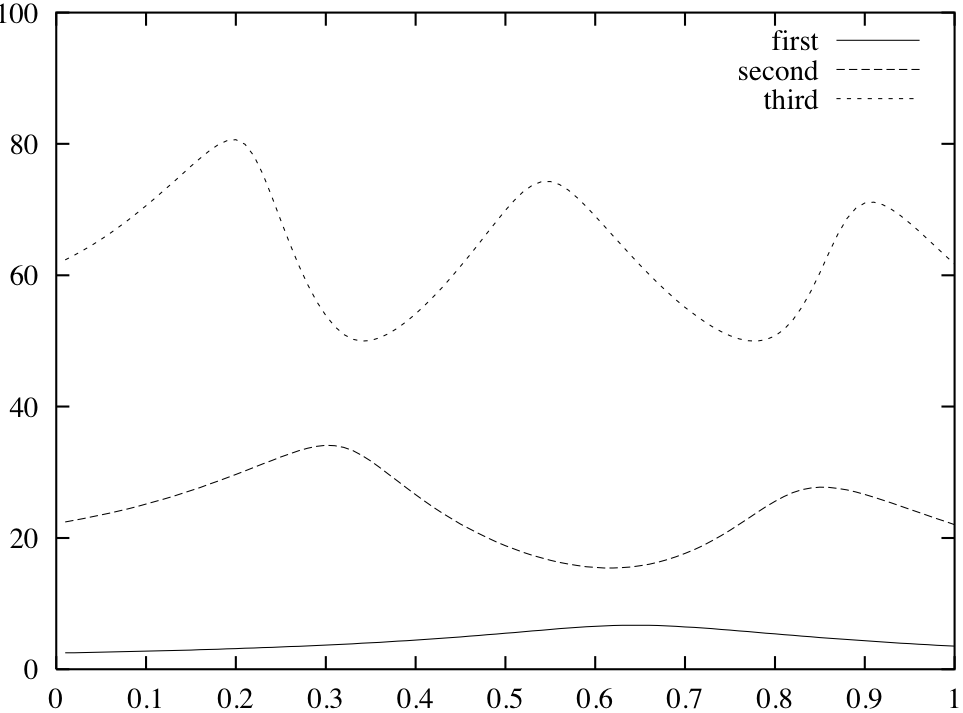
\includegraphics{evolang12.png}}
% \end{center}
% \caption{{\footnotesize An example graph.  All labels are legible, and
%     this caption is in $\backslash$footnotesize. \label{inter}}}
% \end{figure}

% The caption heading for a figure should be placed below that figure.
% The caption text should be $\backslash$footnotesize.

% \section{Supplementary Materials}

% There will be some support for supplementary materials.  All information necessary to understand and evaluate the submission should be included in the main paper.  Reviewers will not see the supplementary materials.  However, authors are encouraged to make data or code available for the final publication.  All supplementary materials should be submitted within a single zip file, which should also include a README.txt file describing the contents.  Supplementary materials should be referenced in the main text (e.g. ``see supplementary materials''). Please avoid appendices in the text and provide additional information in the supplementary materials instead. These will be hosted online along with the final proceedings but will not be considered during the review process.

% \section*{Acknowledgements}

% If you wish to acknowledge funding bodies etc., the acknowledgements may be placed in a separate, unnumbered section at the end of the text. Please replace acknowledgements with filler text for the submission stage to preserve anonymity. Please avoid appendices in the text and provide additional information in the supplementary materials instead. These will be hosted online along with the final proceedings but will not be considered during the review process.
\bibliographystyle{apacite}
\bibliography{evolang12} 

\end{document}
